\section{Auswertung}
\label{sec:Auswertung}

\subsection{Entladung eines Kondensators}

Die aufgenommenen Wertepaare finden sich in Tabelle \ref{tab:Messdaten1}.

\begin{table}
\centering
\caption{Messdaten zur Entladekurve}
\label{tab:Messdaten1}
\sisetup{table-format=2.1}
\begin{tabular}{c c}
\toprule
$t \,/\, \si{\milli\second}$ & $U_C \,/\, \si{\volt}$\\
\midrule
0,00 & 100\\
0,26 &  82\\
0,50 &  70\\
0,76 &  58\\
1,00 &  46\\
1,26 &  38\\
1,50 &  30\\
2,00 &  20\\
3,00 &   6\\
4,10 &   0\\
\bottomrule
\end{tabular}
\end{table} 

Die Wertepaare werden in einem halblogarithmischen Diagramm dargestellt. Dazu 
wird eine lineare Regression mittels Python und matplotlib durchgeführt. Das 
entstandene Diagramm ist in Abbildung \ref{fig:plot1} zu finden. 

\begin{figure}
  \centering
  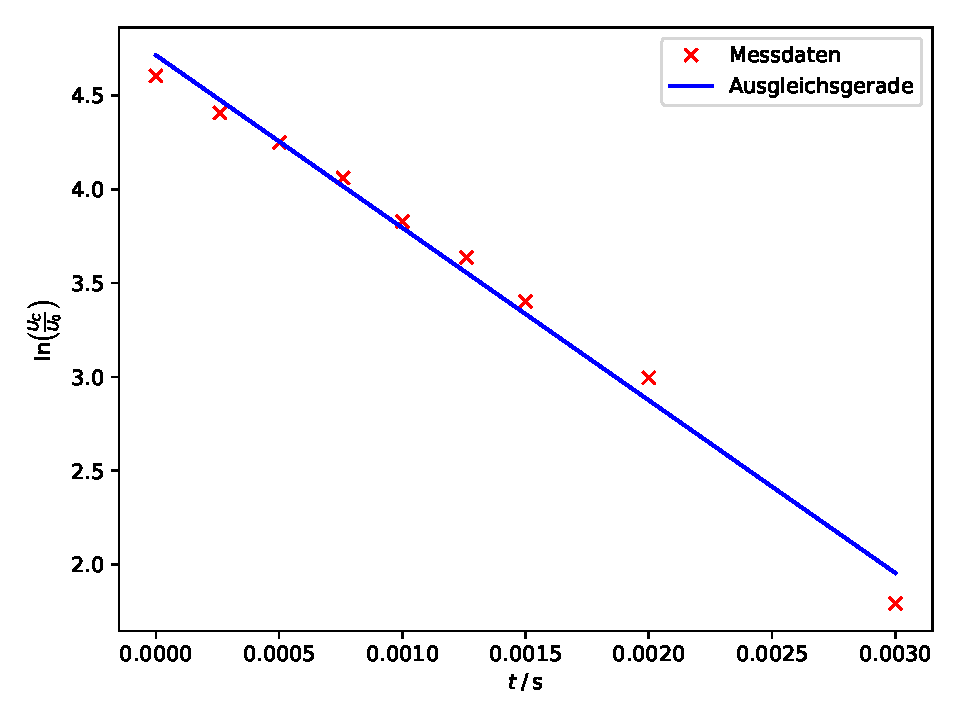
\includegraphics[scale=0.8]{content/plot1.pdf}
  \caption{Lineare Regression zur Bestimmung der Zeitkonstanten mithilfe
  der Entladekurve}
  \label{fig:plot1}
\end{figure}

Die lineare Ausgleichsrechnung der logarithmierten Daten mit $\ln{\left(U_C\right)}=ax+b$ 
ergibt folgende Regressionsparameter: 

\begin{align*}
a &= \SI{-919.67+-45.48}{\per\second},\\
b &= \num{4.71+-0.07}.
\end{align*}

Durch Vergleich mit der Formel \eqref{eqn:ent} ergibt sich für die Zeitkonstante:

\begin{equation*}
RC = -\frac{1}{a} = \SI{1.09+-0.05}{\milli\second}.
\end{equation*}

\subsection{Frequenzabhängigkeit der Amplitude}

In diesem Versuchsteil wird die Frequenzabhängigkeit der Amplitude der 
Kondensatorspannung $U_C$ untersucht. Hierzu wird diese für verschiedene 
Frequenzen $f$ gemessen. Die Messwerte finden sich in Tabelle \ref{tab:Messdaten2}.
Außerdem wird die Amplitude der Generatorspannung zu $U_0=\SI{51.6}{\volt}$ gemessen und 
so das Verhältnis $\frac{A}{U_0}$ für jeden Messwert bestimmt. 

\begin{table}
\centering
\caption{Messdaten zur Frequenzabhängigkeit der Amplitude}
\label{tab:Messdaten2}
\sisetup{table-format=2.1}
\begin{tabular}{c c c}
\toprule
$f \,/\, \si{\hertz}$ & $A \,/\, \si{\volt}$ & $\frac{A}{U_0}$ \\
\midrule
   10 & 49,60 & 0.961\\
   20 & 49,20 & 0.953\\
   30 & 48,00 & 0.930\\
   40 & 46,40 & 0.899\\
   50 & 45,20 & 0.876\\
   60 & 43,60 & 0.845\\
   70 & 42,00 & 0.814\\
   80 & 40,70 & 0.789\\
   90 & 39,20 & 0.760\\
  100 & 37,20 & 0.721\\
  200 & 29,40 & 0.570\\
  300 & 17,60 & 0.341\\
  400 & 13,40 & 0.260\\
  500 & 11,00 & 0.213\\
  600 &  9,10 & 0.176\\
  700 &  7,80 & 0.151\\
  800 &  6,90 & 0.134\\
  900 &  6,30 & 0.122\\
 1000 &  5,60 & 0.109\\
 2000 &  2,76 & 0.053\\
 3000 &  1,84 & 0.036\\
 4000 &  1,40 & 0.027\\
 5000 &  1,12 & 0.022\\
 6000 &  0,92 & 0.018\\
 7000 &  0,80 & 0.016\\
 8000 &  0,71 & 0.014\\
 9000 &  0,62 & 0.012\\
10000 &  0,56 & 0.011\\
\bottomrule
\end{tabular}
\end{table} 

Stellt man diese Werte graphisch da, so ergibt sich Abbildung ... .

%\begin{figure}
%  \centering
%  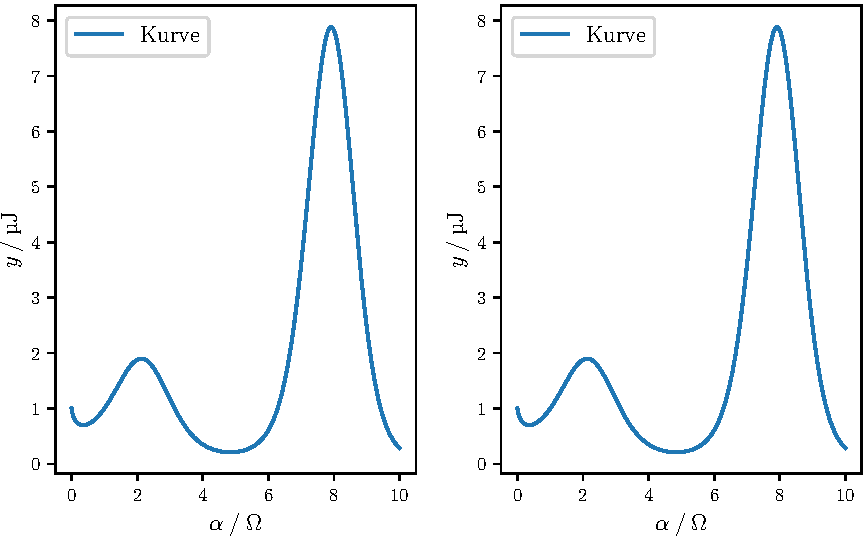
\includegraphics{plot.pdf}
%  \caption{Plot.}
%  \label{fig:plot}
%\end{figure}
